\documentclass[xcolor=dvipsnames]{beamer}

\usepackage[utf8]{inputenc}
\usepackage[english]{babel}
\usepackage[T1]{fontenc}
\usepackage{xcolor}

\usepackage{amsmath}
\usepackage{amssymb}
\usepackage{amsfonts}
\usepackage{times}
\usepackage{autobreak}
\usepackage{relsize}
\usepackage{enumerate}
\usepackage{booktabs}
\usepackage{color}
\usepackage{xcolor}
\usepackage{graphicx}
\usepackage{epstopdf}
\usepackage{float}
\usepackage{placeins}
\usepackage[caption=false]{subfig}
\usepackage{hyperref}
\usepackage[toc,page]{appendix}

\graphicspath{./image/}

%%%%%%%%%%%%%%%%%%%%%%%%%%%%%%%%%%%%%%%%
\usetheme{Berlin}
%\usecolortheme[named=Blue]{structure}

\definecolor{lightgray}{gray}{0.95}
\definecolor{myellow}{RGB}{255,255,0}
\setbeamercolor{background canvas}{bg=lightgray}
\setbeamercolor{section in head/foot}{fg=white}
\setbeamercolor{title}{fg=myellow}
\setbeamercolor{frametitle}{fg=myellow}
\setbeamercolor{block title}{fg=white}

\usefonttheme{structurebold}

\useinnertheme{circles}
\useinnertheme{rounded}

\makeatletter
\setbeamertemplate{headline}{
  \begin{beamercolorbox}[ht=2.25ex,dp=2.85ex]{section in head/foot}
    \insertnavigation{\paperwidth}
  \end{beamercolorbox}
}

\setbeamertemplate{frametitle}{
  \nointerlineskip
  \begin{beamercolorbox}[sep=0.4ex,wd=\paperwidth]{frametitle}
    \vskip-0.5ex
    \strut\insertframetitle\strut
  \end{beamercolorbox}
}
\makeatother

\usepackage{appendixnumberbeamer}

\definecolor{H1}{RGB}{238,0,0}
\definecolor{L1}{RGB}{75,166,255}

%%%%%%%%%%%%%%%%%%%%%%%%%%%%%%%%%%%%%%%%
\title[Introduction to Gravitational Wave Data Analysis]
{Introduction to Gravitational Wave Data Analysis}

\author[Chia-Jui Chou]
{\Large{Chia-Jui Chou}}

\institute[2025/04/17]
{National Yang Ming Chiao Tung University, Taiwan}

\date[2025/04/17]
{}

%%%%%%%%%%%%%%%%%%%%%%%%%%%%%%%%%%%%%%%%
\begin{document}

\begin{frame}
  \titlepage
\end{frame}

% \begin{frame}{Outline} \label{outline}
  % \tableofcontents
% \end{frame}

\setcounter{equation}{0}
\renewcommand{\theequation}{\arabic{section}.\arabic{equation}}

%%%%%%%%%%%%%%%%%%%%%%%%%%%%%%%%%%%%%%%%
\section[GW]{Gravitational Wave}

\begin{frame}[t]{General Relativity: Einstein Equation}
  \begin{block}{Einstein Equation}
    \begin{equation*}
      R_{\mu\nu} - \frac{R}{2} g_{\mu\nu} = \frac{8\pi G}{c^4} T_{\mu\nu},
    \end{equation*}
  \end{block}
  \begin{itemize}
    \item $g_{\mu\nu}$: metric tensor,
    \item $R_{\mu\nu}$: Ricci tensor,
    \item $R = g^{\mu\nu} R_{\mu\nu}$: Ricci scalar,
    \item $T_{\mu\nu}$: stress-energy tensor.
  \end{itemize}
  \begin{block}{Measure of interval in spacetime}
    \begin{equation*}
      ds^2 = g_{\mu\nu} dx^\mu dx^\nu.
    \end{equation*}
  \end{block}
\end{frame}

\begin{frame}[t]{General Relativity: Linearized Theory}
  \begin{block}{Perturbation of metric tensor}
    \begin{equation*}
      g_{\mu\nu} = \eta_{\mu\nu} + h_{\mu\nu}, \quad |h_{\mu\nu}| \ll 1.
    \end{equation*}
  \end{block}
  \begin{block}{Linearized Einstein Equation}
    \begin{equation*}
      \Box \bar{h}_{\mu\nu} + \eta_{\mu\nu} \partial^\rho \partial^\sigma \bar{h}_{\rho\sigma} - \partial^\rho \partial_\nu \bar{h}_{\mu\rho} - \partial^\sigma \partial_\mu \bar{h}_{\nu\rho} = -\frac{16\pi G}{c^4} T_{\mu\nu}.
    \end{equation*}
  \end{block}
  \begin{itemize}
    \item $h = \eta^{\mu\nu} h_{\mu\nu}$,
    \item $\bar{h}_{\mu\nu} = h_{\mu\nu} - \frac{1}{2} \eta_{\mu\nu} h$.
  \end{itemize}
\end{frame}

\begin{frame}[t]{Harmonic Gauge and Transverse-Traceless Gauge}
  \begin{block}{Harmonic Gauge}
    \begin{equation*}
      \partial^\nu \bar{h}_{\mu\nu} = 0.
    \end{equation*}
  \end{block}
  \begin{block}{Linearized Einstein Equation}
    \begin{equation*}
      \Box \bar{h}_{\mu\nu} = 0,
    \end{equation*}
  \end{block}
  $T_{\mu\nu} = 0$ if we observe the GW far away from the source.
  \begin{block}{Transverse-Traceless Gauge}
    \begin{equation*}
      h^{0\mu}, \quad h^i_i = 0, \partial^j h_{ij} = 0,
    \end{equation*}
  \end{block}
  which can only be chosen away from the source.
\end{frame}

\begin{frame}[t]{Solution of the Gravitational Wave}
  We can choose the propagation direction along $\hat{z}$, with the wave vector:
  \begin{equation*}
    k^\mu = (\omega/c, \mathbf{k}),
  \end{equation*}
  and the solution of GW:
  \begin{equation*}
    h^{\text{TT}}_{\mu\nu} (t, z) =
    \begin{pmatrix}
      0 & 0 & 0 & 0 \\
      0 & h_{+} & h_{\times} & 0 \\
      0 & h_{\times} & -h_{+} & 0 \\
      0 & 0 & 0 & 0
    \end{pmatrix}
    \cos \left[ \omega(t - z/c) \right].
  \end{equation*}
  The we have the perturbed metric tensor:
  \begin{align*}
    ds^2 = & -c^2 dt^2 + dz^2 + \left\{ 1 + h_{+}\cos[\omega(t - z/c)] \right\} dx^2 \\
    & - \left\{ 1 + h_{+}\cos[\omega(t - z/c)] \right\} dy^2 + 2h_{\times}\cos[\omega(t - z/c)] dxdy.
  \end{align*}
\end{frame}

\begin{frame}[t]{Gravitational Wave Interacting with Test Masses}
  \begin{center}
    \includegraphics[width=\textwidth]{image/test-mass.png}
  \end{center}
\end{frame}

\begin{frame}[t]{Gravitational Wave Detector}
  \begin{center}
    \includegraphics[height=0.8\textheight]{./image/GW-detector.png}
  \end{center}
\end{frame}

\begin{frame}[t]{Gravitational Wave Detector}
  \begin{center}
    \includegraphics[height=0.8\textheight]{./image/KAGRA_IFO.png}
  \end{center}
\end{frame}

\begin{frame}[t]{Gravitational Wave Detector}
  \begin{equation*}
    0 = -c^2 dt^2 + \left( 1 + h_+ \right) dx^2, \quad \rightarrow cdt \simeq \left( 1 + \frac{h_+}{2} \right) \left| dx \right|.
  \end{equation*}
  \begin{equation*}
    \Delta T_x = \frac{h_+ L_x}{2c}, \quad \Delta L_x = \frac{h_+ L_x}{2}.
  \end{equation*}
  \begin{equation*}
    0 = -c^2 dt^2 + \left( 1 - h_+ \right) dy^2, \quad \rightarrow cdt \simeq \left( 1 - \frac{h_+}{2} \right) \left| dy \right|.
  \end{equation*}
  \begin{equation*}
    \Delta T_y = -\frac{h_+ L_y}{2c}, \quad \Delta L_y = -\frac{h_+ L_y}{2}.
  \end{equation*}
  \begin{equation*}
    \Delta L = \Delta L_x - \Delta L_y = h_+ \cdot \frac{L_x + L_y}{2} \equiv h_+ L.
  \end{equation*}
\end{frame}

\begin{frame}[t]{Gravitational Wave Detectors}
  \begin{center}
    \includegraphics[width=\textwidth]{image/GW_Detector_Map.jpg}
  \end{center}
\end{frame}

\begin{frame}[t]{Observation Runs}
  \begin{center}
    \includegraphics[width=\textwidth]{image/ObsScen_timeline.png}
  \end{center}
\end{frame}

\begin{frame}[t]{Multi-Messenger Astronomy (MMA)}
  \begin{center}
    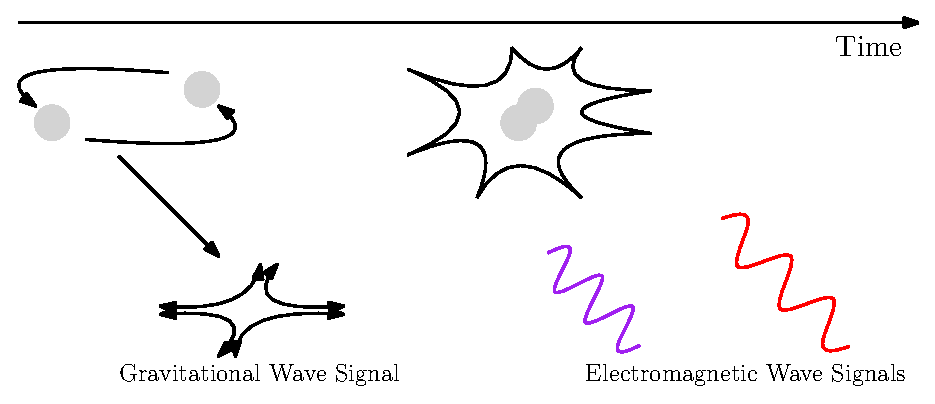
\includegraphics[width=0.9\textwidth]{image/BNS-MMA.eps}
  \end{center}
  Sky localization of the {\color{blue}"Known GW Sources"} from their GW signals and send out alerts in low latency for the EM telescopes to capture the follow-up EM wave signals.
\end{frame}

\begin{frame}[t]{Sources of Gravitational Waves}
  \begin{itemize}
    \item {\color{orange}Compact Binary Coalescence}:
    \begin{itemize}
      \item Black Hole-Black Hole Mergers,
      \item Neutron Star-Neutron Star Mergers,
      \item Black Hole-Neutron Star Mergers.
    \end{itemize}
    \item {\color{green}Bursts}:
    \begin{itemize}
      \item Core-collapse Supernovae, Fast Radio Burst, Gamma Ray Burst, etc.
    \end{itemize}
    \item {\color{blue}Continuous Waves}:
    \begin{itemize}
      \item Spinning Neutron Stars,etc.
    \end{itemize}
    \item Stochastic Background:
    \begin{itemize}
      \item Cosmological background, Astrophysical background, etc.
    \end{itemize}
  \end{itemize}
\end{frame}

%%%%%%%%%%%%%%%%%%%%%%%%%%%%%%%%%%%%%%%%
\section[GW Data]{Gravitational Wave Data}

\begin{frame}[t]{Gravitational Waveforms and Background Noise}
  GW strain: $h(t) = \frac{\Delta L(t)}{L} \sim 10^{-22}$.
  \begin{center}
    \includegraphics[height=0.3\textheight]{./image/BBH_signal-H1.png}
    \includegraphics[height=0.3\textheight]{./image/BBH_ts-H1.png}
  \end{center}
\end{frame}

\begin{frame}[t]{Power Spectral Density (PSD)}
  \begin{center}
    \includegraphics[width=0.8\textwidth]{image/PSD_H1-1266281937-128.png}
  \end{center}
\end{frame}

\begin{frame}[t]{Finding BBH Signals}
  \begin{center}
    \includegraphics[width=0.8\textwidth]{image/BBH_whiten_ts_H1.png}
    \includegraphics[width=0.8\textwidth]{image/Correlation_ts_H1.png}
  \end{center}
\end{frame}

\begin{frame}[t]{Finding BBH Signals (Matched Filtering)}
  \begin{center}
    \includegraphics[width=0.8\textwidth]{image/Correlation_ts_H1.png}
    \includegraphics[width=0.8\textwidth]{image/Spectrogram_BBH_H1.png}
  \end{center}
\end{frame}

\begin{frame}[t]{Glitches (Matched Filtering)}
  \begin{center}
    \includegraphics[width=0.8\textwidth]{image/Correlation_ts_Glitch_H1.png}
    \includegraphics[width=0.8\textwidth]{image/Spectrogram_Glitch_H1.png}
  \end{center}
\end{frame}

\begin{frame}[c]{}
  \begin{center}
    \includegraphics[scale=0.5]{image/Thankyou.png}
  \end{center}
\end{frame}

%%%%%%%%%%%%%%%%%%%%%%%%%%%%%%%%%%%%%%%%
% \appendix
% \section{Appendices}

\end{document}